\documentclass{article}
\usepackage{iclr2025_conference,times}
\usepackage{hyperref}
\usepackage{url}
\usepackage{enumitem}
\usepackage{booktabs}
\usepackage{titlesec}
\usepackage{float}
\usepackage{graphicx}
\titlespacing\section{0pt}{4pt}{2pt}
\titlespacing\subsection{0pt}{2pt}{1pt}
\title{Bon Voyage Bot: An Agentic Conversational AI System for Personalized Travel Planning}
\author{Sydney Smith  \\
ECE 57000 | Purdue University\\
\texttt{smit6806@purdue.edu} \\
}
\newcommand{\fix}{\marginpar{FIX}}
\newcommand{\new}{\marginpar{NEW}}
\iclrfinalcopy

\begin{document}
\maketitle

\begin{abstract}
Travelers today face a fragmented and time-consuming planning process, navigating disconnected platforms such as search engines, flight aggregators, and hotel booking sites that neither share context nor adapt to individual needs. This paper presents Bon Voyage Bot, a conversational artificial intelligence (AI) agent designed to personalize the travel planning process by enabling users to build an itinerary through natural language conversation within a single intelligent interface. The system is built for travelers who desire a streamlined planning experience that is both adaptive and conversational. Bon Voyage Bot is implemented as a web application powered by large language model (LLM) technology that extracts trip details and user preferences from conversation and maintains them in a structured schema that persists throughout the session. A rule-based routing mechanism uses the schema to determine when sufficient information is available to invoke external APIs. The model can autonomously retrieve real-world information, such as flight options, hotel availability, restaurant recommendations, and local attractions, all at the appropriate moments in the conversation. The user can interactively refine their plan through dialog and download a complete travel itinerary that consolidates all planning outputs. The prototype was evaluated against user-defined success criteria, including maintaining conversational context, accurately extracting structured trip specifications, and delivering personalized recommendations grounded in live data. Results demonstrated that the system successfully met these criteria. These findings highlight the potential of agentic LLM architectures for addressing complex, real-world planning tasks.
\begin{center}
    \href{https://github.com/smit6806/bon-voyage-bot}{Code and LaTeX Source}
\end{center}
\end{abstract}

\section{Introduction}
Travel planning is a time-consuming and demanding process. Users must balance qualitative constraints such as personal preferences with quantitative requirements, including budget and scheduling, while navigating a disjointed landscape of digital tools. The burden of synthesizing information into a cohesive plan falls entirely on the user, contributing to decision fatigue and reducing the overall quality of the planning experience \citep{greenwood2020}. While human travel planners offer personalized recommendations and alleviate some of these concerns, their services are often limited by cost, availability, and scalability. 

Recent advancements in artificial intelligence have produced systems capable of sophisticated reasoning, natural language understanding, and autonomous decision-making. However, the tools available have yet to incorporate these capabilities meaningfully into the travel planning domain. Standard LLM-based conversational systems are limited in their ability to reliably store information and integrate real-world data sources \citep{schick2023toolformer}. Without these capabilities, systems struggle to move beyond generic suggestions, leaving a clear gap for a more capable unified solution \citep{shivakumar2025}.

International tourism reached a record 1.52 billion arrivals globally in 2025 \citep{unwto2026}, reflecting sustained and growing demand for travel worldwide. At the same time, the travel sector contributed an unprecedented \$11.6 trillion to the global economy \citep{wttc2025}, underscoring the scale and significance of the industry. Together, these figures highlight that demand for intelligent, personalized travel planning tools has never been greater. This work presents Bon Voyage Bot, a conversational AI agent that addresses the limitations of existing tools through a personalized, dialog-driven travel planning interface powered by large language model technology, structured data management, and real-world API integration. By consolidating the fragmented travel planning process into a single conversational interface, Bon Voyage Bot aims to reduce the burden on users and deliver a planning experience that is both adaptive and grounded in live data.  

The key contributions of this work are as follows:
\begin{itemize}[noitemsep, topsep=0pt]
    \item A conversational AI travel planning agent hosted through a single intelligent interface.
    \item A two-tier decision architecture combining rule-based tool routing with LLM-driven function calling to ground system responses in real-world data.
    \item A structured state management approach that progressively captures trip specifications across multi-turn conversations.
    \item A background itinerary generation system that builds a downloadable travel document in parallel with the conversation without impacting response latency.
    \item A functional end-to-end prototype demonstrating the viability of agentic LLM architectures for real-world planning tasks.
\end{itemize}

\section{Problem Definition and User Requirements}
\label{sec:problem}

\subsection{Problem Definition}
Travel planning is a complex, multi-step task that requires users to coordinate information across a wide range of platforms and services. Despite the availability of numerous digital tools, no single platform currently provides an end-to-end solution that adapts to individual user needs, maintains context across an entire planning session, and integrates real-world data in a conversational and personalized manner. This gap motivates the development of an intelligent, agentic system that can unify the planning process and reduce the burden placed on the user. 

\subsection{Target User}
Bon Voyage Bot is designed for casual travelers planning domestic or international trips, regardless of group size or composition. The target user is someone who lacks the time for extensive manual research, finds existing tools fragmented and difficult to navigate, and desires a planning experience that is both adaptive and conversational.

\subsection{User Requirements}
A successful system must satisfy the following requirements from the perspective of the target user:
\begin{itemize}[noitemsep, topsep=0pt]
    \item Accept natural language input without requiring structured forms or rigid workflows
    \item Maintain context and trip details across multiple conversation turns
    \item Retrieve real-world information including flights, hotels, restaurants, and local attractions
    \item Provide personalized recommendations based on budget, preferences, and travel dates
    \item Allow the user to iteratively refine their plan through dialog
    \item Generate a consolidated, downloadable itinerary as a final output
\end{itemize}

\subsection{Success Criteria}
The system will be considered successful if it satisfies the following criteria, each of which directly corresponds to a user requirement identified in the previous subsection.
\begin{itemize}[noitemsep, topsep=0pt]
    \item \textbf{Contextual extraction:} The system extracts and maintains structured trip specifications from conversation, including origin, destination, dates, budget, and preferences.
    \item \textbf{Intelligent API invocation:} The system correctly determines when sufficient trip context has been established and autonomously invokes external APIs to retrieve real-world data.
    \item \textbf{Personalized itinerary generation:} The system produces a day-by-day itinerary and allows the user to refine the plan through continued dialog.
    \item \textbf{Consolidated output:} The system generates a downloadable itinerary document that consolidates all planning outputs into a single document for reference and use.
\end{itemize}

These criteria are qualitatively evaluated through structured test conversations designed to exercise each component of the system. Each test scenario provides a representative set of trip details through natural dialog and assesses whether the system responds appropriately at each stage of the interaction. The results of this evaluation are presented in Section \ref{sec:results}.


\section{Related Work}
\label{sec:related}

\subsection{Conversational AI and Large Language Models}
The development of large language models has fundamentally transformed the capabilities of conversational AI systems. Early conversational agents such as ELIZA and rule-based chatbots were limited to pattern matching and scripted responses, requiring extensive hand-crafted logic for each domain \citep{wang2023survey}. The introduction of neural network-based approaches, and more recently, transformer architectures enabled a new generation of systems capable of open-ended natural language understanding and generation. Models such as GPT-4 demonstrate strong performance across a wide range of language tasks, from question answering to code generation, and have been widely adopted as the backbone of modern conversational applications \citep{openai2023gpt4}. However, standard LLM-based conversational systems face notable limitations when applied to complex tasks. They lack persistent memory throughout a conversation, making it difficult to track evolving user requirements over multiple turns. They cannot maintain structured representations of data, meaning that details mentioned early in a conversation may be lost or misinterpreted later. They also cannot access real-time external data sources without explicit augmentation \citep{schick2023toolformer}. Bon Voyage Bot addresses these limitations through structured state management and tool-augmented function calling, which are described in detail in Section \ref{sec:system}.

\subsection{AI in Travel and Tourism}
The application of artificial intelligence, machine learning, and natural language processing into travel platforms has significantly enhanced their functionality, enabling features such as dynamic itinerary generation, personalized recommendations, and conversational interfaces \citep{shivakumar2025}. While recommendation systems can suggest destinations and activities based on user preferences and historical behavior, they tend to be static, generating recommendations from predefined user profiles rather than adapting through natural language. 
More recently, large language models have been explored for intelligent travel planning. Google Research demonstrated a hybrid approach combining LLM-generated itineraries with optimization algorithms to handle real-world constraints including opening hours and travel times, noting that LLMs alone struggle with quantitative logistical requirements \citep{google2024tripplanning}. This limitation is further evidenced by TravelPlanner, a benchmark study showing that GPT-4 achieves a success rate of only 0.6\% on complex travel planning tasks that require satisfying multiple real-world constraints \citep{xie2024travelplanner}. Bon Voyage Bot's solution advances beyond these approaches by maintaining a persistent validated trip profile that evolves throughout the conversation and grounds recommendations in live external data. 


\subsection{Tool-Augmented LLMs and Agentic Architectures}
The integration of external tools with large language models has emerged as a promising direction for extending LLM capabilities beyond static knowledge. Schick et al. introduced Toolformer, demonstrating that language models can learn to invoke external APIs autonomously through self-supervised training, deciding when to call tools, what arguments to pass, and how to incorporate results into their responses \citep{schick2023toolformer}. Yao et al. proposed ReAct, a framework that combines reasoning traces with external tool use, enabling language models to dynamically update their action plans based on real-world feedback \citep{yao2023react}. OpenAI's function calling mechanism extended this concept, enabling models to invoke predefined functions based on conversational context \citep{openai2023gpt4}. However, most tool-augmented systems invoke tools reactively based solely on conversational context, without a structured state layer to control API access or verify that sufficient information exists to produce meaningful results. Bon Voyage Bot introduces a two-tier decision architecture that combines rule-based tool routing with LLM-driven function calling, ensuring that external APIs are only invoked when the structured data schema contains sufficient context. This approach reduces unnecessary API calls and improves the reliability of results.

\subsection{Structured State Management in Dialog Systems}
A core challenge in building intelligent conversational agents is maintaining a coherent understanding of user goals and requirements across multiple interaction turns. Task-oriented conversational systems have long addressed this through structured tracking mechanisms that monitor user intent and relevant constraints as they emerge across conversation turns \citep{wang2023survey}. However, these approaches typically require domain-specific training data and are limited to narrow, predefined task structures. Recent language model systems rely on the conversation history as a record of user requirements, which can be unreliable for complex planning tasks where precise constraint tracking is essential \citep{xie2024travelplanner}. Bon Voyage Bot addresses this limitation by introducing a structured validation schema that is explicitly populated and validated at each conversation turn, providing a reliable and updated representation of trip specifications. This schema serves as the foundation for API routing and personalized recommendation generation. 


\section{Methodology}
\label{sec:system}

\subsection{System Overview}
Bon Voyage Bot is implemented as a modular, web-based conversational agent built on top of the OpenAI GPT-4o API and deployed using the Streamlit framework. The system follows an agentic architecture in which a central Agent Orchestrator manages all aspects of the interaction, including prompt construction, structured state management, and tool routing. The architecture is organized across three layers: a front-end user interface layer, an agentic logic layer, and an external services layer. A high-level overview of the system architecture is shown in Figure \ref{fig:architecture}.
\begin{figure}[H]
    \centering
    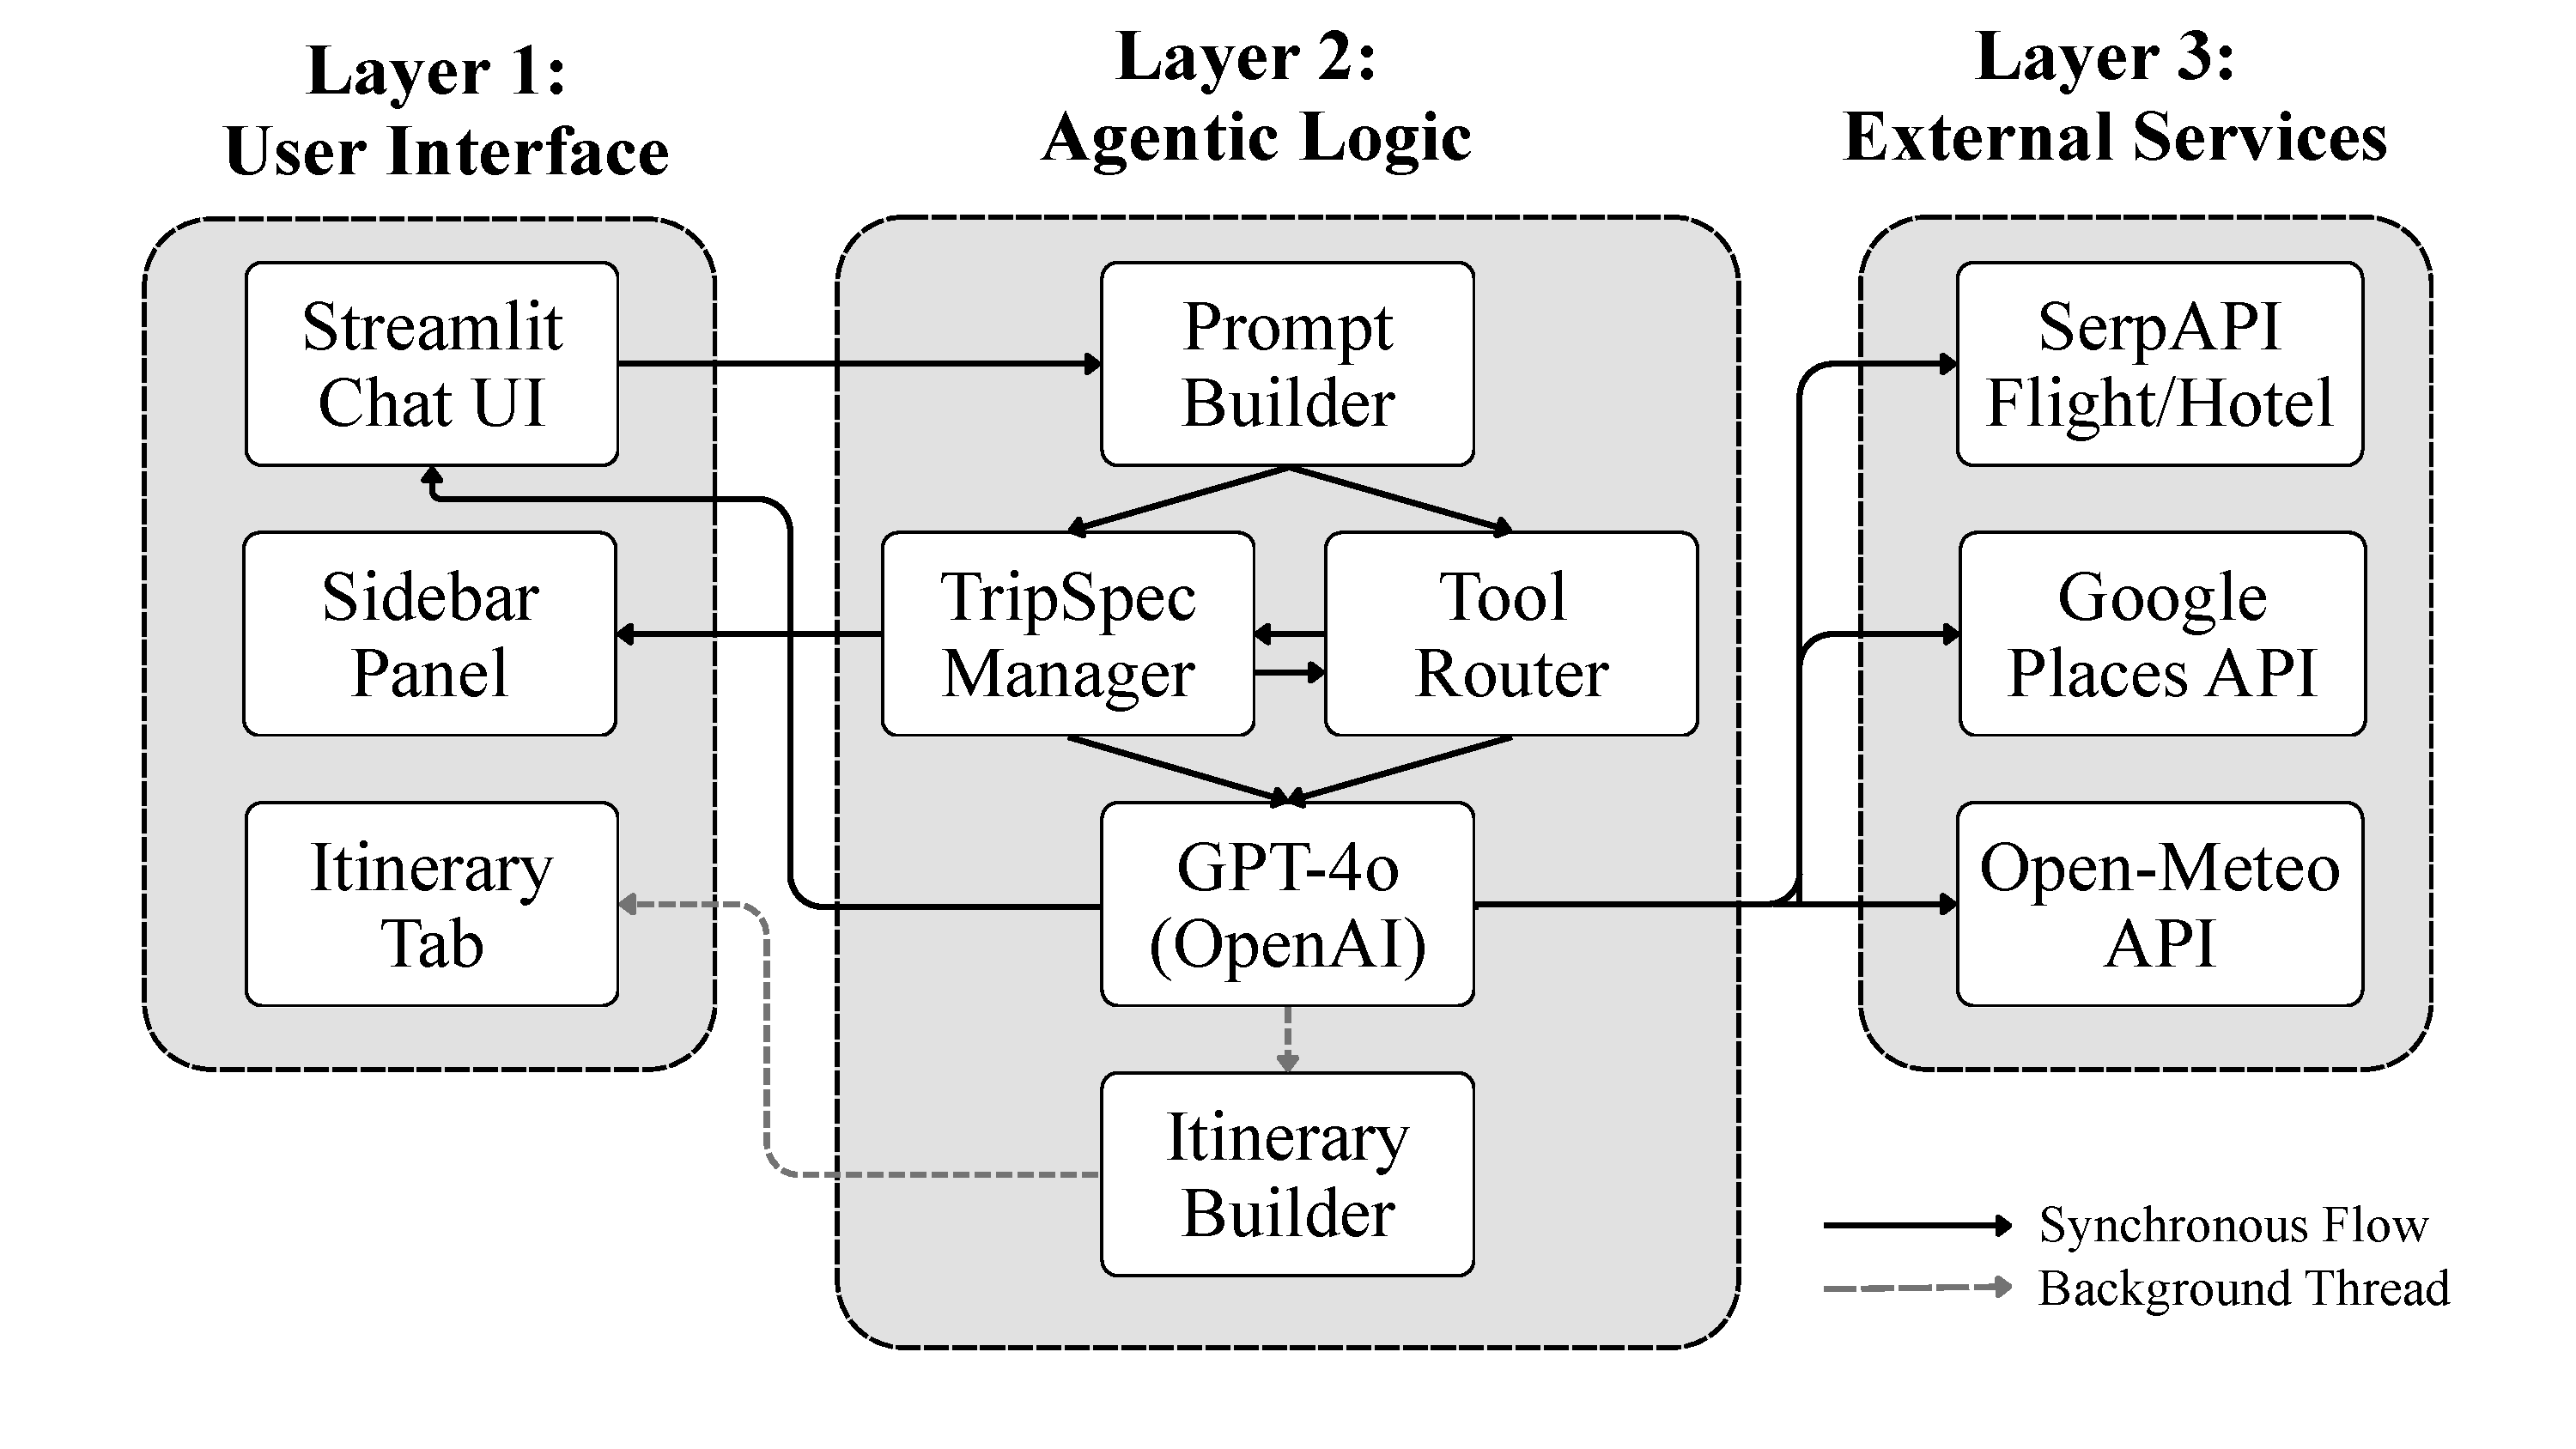
\includegraphics[width=.9\linewidth]{Bon Voyage Bot System Architecture.pdf}
    \caption{System architecture of Bon Voyage Bot across three layers}
    \label{fig:architecture}
\end{figure}

\subsection{Conversational Interface}
The user interface is implemented as a Streamlit web application featuring a chat-style input and response display. User messages are captured through a text input field and appended to a persistent conversation history that is maintained in Streamlit session state across interaction turns. The full conversation history is passed to the language model at each turn, ensuring that responses remain contextually coherent throughout the session. A sidebar panel displays a real-time summary of the structured trip details extracted from the conversation, including origin, destination, travel dates, budget, and user preferences, along with typical historical weather conditions for the travel month and a live budget tracker that updates as flights and hotels are confirmed. A dedicated Itinerary tab displays the travel document as it builds in the background and provides a button to export the finalized plan as a PDF.

\subsection{Structured State Management}
The system employs a structured validation schema, referred to as TripSpec, implemented using the Pydantic data validation library for Python. TripSpec defines a hierarchical set of fields capturing all relevant trip attributes, including origin city and airport code, destination city and region, travel dates and duration, traveler count, budget constraints, and user preferences such as trip type, pace, and luxury level. At each conversation turn, the full conversation history is passed to GPT-4o alongside a dedicated extraction prompt that instructs the model to return a JSON object conforming to the TripSpec structure. The extracted data is validated by Pydantic before being merged with the existing TripSpec instance, ensuring that only well-formed data persists across the session. This approach provides a reliable and continuously updated structured representation of the user's trip requirements that is available to all other system components. 

\subsection{Prompt Engineering}
Prompt design plays a central role in the reliability of the system. Two primary prompts govern the behavior of the language model, each serving a distinct purpose. The system prompt defines the persona and behavioral guidelines of Bon Voyage Bot, instructing GPT-4o to gather trip details through natural conversational questioning, ask no more than one or two questions at a time, and prioritize budget-conscious recommendations throughout the interaction. The extraction prompt is kept separate from the system prompt by design, as combining the two risks compromising both the conversational response quality and the accuracy of structured extraction. Instead, the extraction prompt instructs GPT-4o to return only a valid JSON object matching the TripSpec structure, specifying rules such as usage of null values for unmentioned fields and interpreting ambiguous dates relative to the current date. The extraction prompt, combined with the validated Pydantic schema, TripSpec, allows the model to maintain a structured representation of the interaction. 

\subsection{Tool Router}
The Tool Router is a rule-based component that evaluates the completeness of the current TripSpec instance to determine which external APIs have sufficient information to return meaningful results. Boolean conditions are evaluated at each turn based on the presence of key fields: origin city, destination city, travel dates or duration, and traveler count. Based on these conditions, the Tool Router returns a list of API identifiers that are ready to be invoked. The Google Places API is enabled as soon as a destination is known, flight search requires origin, destination, dates, and traveler count, and hotel search requires destination and dates. This gating mechanism ensures that API calls are only made when sufficient context exists to produce useful output. 

\subsection{Function Calling and API Integration}
External API access is mediated through OpenAI function calling, which allows GPT-4o to autonomously decide when and what to query from external services based on conversational context and the available tool definitions. The Tool Router determines which tool definitions are passed to GPT-4o at each turn, ensuring that the model only has access to APIs that are ready to return meaningful results. Flight and hotel searches are powered by the SerpAPI Google Flights and Google Hotels engines respectively, while place and activity recommendations are retrieved through the Google Places API. Historical weather conditions for the travel destination and month are retrieved from the Open-Meteo climate API, which requires no authentication and provides monthly temperature and precipitation averages.

\subsection{Itinerary Generation}
The system generates a travel itinerary document continuously in the background as the user converses, using a dedicated background thread that runs after every user message without blocking the chat interface. The background process makes two sequential LLM calls: the first extracts confirmed bookings and action items as structured JSON for budget tracking and the bookings display in the sidebar, and the second generates a free-form markdown narrative of the day-by-day plan based only on what has been explicitly confirmed in the conversation. Results are communicated back to the main thread via a Python queue to avoid Streamlit session state concurrency issues. The final itinerary is rendered in a dedicated tab and exported as a formatted PDF using the ReportLab library.


\section{Experimental Results and Analysis}
\label{sec:results}
\begin{table}[h]
\centering
\caption{Evaluation results across four structured test scenarios.}
\label{tab:results}
\begin{tabular}{p{2.2cm}p{2.2cm}p{9cm}c}
\toprule
\textbf{Scenario} & \textbf{Criteria} & \textbf{Key Observations} \\
\midrule
Domestic \newline round-trip & Contextual \newline extraction & TripSpec segments including origin, destination, dates, and budget captured within one to two turns, maintained in sidebar panel \\
\addlinespace
International multi-city & State \newline management & Multiple TripSpec segments created, hotel searches presented sequentially, and itinerary updated properly with multiple cities\\
\addlinespace
Iterative\newline refinement & API \newline invocation & Proper API calls driven by follow-up dialog, including selecting new dates, updating flights, new hotels, and different activities  \\
\addlinespace
Full trip \newline planning & Itinerary \newline generation & Itinerary updated after each turn with no impact on response latency, reflected only confirmed details, PDF exported cleanly  \\
\bottomrule
\end{tabular}
\end{table}
The prototype was evaluated through four structured test conversations, each targeting a success criterion from Section \ref{sec:problem}, with results summarized in Table \ref{tab:results}. Across all scenarios, the system successfully extracted and maintained structured trip specifications from natural language input, with origin, destination, dates, traveler count, and preferences consistently captured within one to two turns. The Tool Router correctly gated API access in all cases, with no unnecessary calls observed. In the multi-city scenario, the system populated stay segments correctly and presented hotel searches sequentially. The background itinerary generation system performed as intended with no observable impact on response latency, and generated narratives contained no hallucinated content. The PDF export rendered cleanly across all test cases.

The iterative refinement scenario demonstrated the system's ability to adapt to changing user requirements mid-conversation. When the user updated travel dates, the system correctly re-extracted the new dates into the TripSpec schema, updated the sidebar, and invoked new flight and hotel searches reflecting the revised parameters without losing previously confirmed preferences. The conversational context was preserved throughout, and the itinerary document updated accordingly after each turn. Across all scenarios, the two-tier decision architecture proved effective; the rule-based Tool Router ensured APIs were only called when sufficient context existed, while GPT-4o's function calling handled the judgment of when and what to query within those bounds. Together, these components produced a system that demonstrated responsiveness and contextual coherence throughout the planning session.

\section{Conclusion}
\label{sec:conclusion}
This paper presented Bon Voyage Bot, a conversational AI travel planning agent that addresses the fragmentation and context loss inherent in existing digital travel tools. The system demonstrates that a structured state management approach, combined with rule-based tool routing and LLM-driven function calling, can produce a reliable and personalized travel planning experience grounded in real-world data. The prototype successfully satisfied all success criteria defined in Section \ref{sec:problem}: structured trip specifications were consistently extracted and maintained across conversations, external APIs were invoked at the correct moments, personalized itineraries were generated and refined through continued dialog, and a downloadable PDF itinerary was produced as a consolidated planning artifact. As a product prototype contribution, this work demonstrates the end-to-end engineering of an agentic LLM application from problem definition to deployed prototype. The key technical contributions include the two-tier decision architecture separating rule-based routing from LLM function calling, the Pydantic-validated trip schema for reliable state management, and the background itinerary generation system. 

Future work could explore the following concepts: 
\begin{itemize}[noitemsep, topsep=0pt]
    \item Replace the rule-based Tool Router with a learned routing policy.
    \item Incorporate user feedback signals to improve personalized recommendations over time.
    \item Support booking and transaction workflows beyond the current recommendation-only scope.
\end{itemize}
 

\bibliography{iclr2025_conference}
\bibliographystyle{iclr2025_conference}

\appendix
\section*{LLM Acknowledgement}
Large language model assistance was used in the preparation of this work. Claude (Anthropic) was used throughout the writing process to provide feedback on grammar, clarity, academic tone, and structural organization of the paper, and assisted in drafting this acknowledgement section. Grammarly's AI writing assistant was used during the initial drafting phase to support grammar and style corrections. The author reviewed and approved all suggested changes, and all technical content, code, and experimental results reflect the author's own work. A full transcript of the Claude-assisted editing session is available below.
\begin{center}
    \href{https://claude.ai/chat/8d8c36b4-2fe5-4fe7-ad06-7cf96ae51a00}{Link to Claude conversation}
\end{center}

\end{document}
